\subsection{Rangefinder Operation}
Because this device is intended to traverse unknown locations and create a 2-dimensional map, data accuracy, precision, and reliability are vital. As such, proper equipment is needed to suffice these needs. 

\subsubsection{Rangefinder Selection}
The project's rangefinder selection depended on the following criteria: field of vision, depth of sense, accuracy, precision, and cost. Many of the rangefinders limited by our budgetary restrictions were only strong in one of our project's vital criteria. However Professor Duckworth, and WPI's Electrical and Computer Engineering and Robotics Engineering Departments generously donated the URG-04LX Scanning Laser Rangefinder for the purpose of this project. The URG-04LX is a very sensitive piece of equipment that has a field of view of 240 degrees, a depth of data of 4 meters, and accuracy to within 10 millimeters, which is perfect for our application \cite{urg04lx_specifications}. Figure \ref{rangefinder_pic} below shows the URG-04LX rangefinder that we will be using.

\begin{figure}[H]
	\centerline{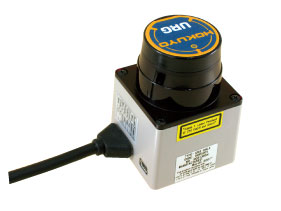
\includegraphics[width=0.5\textwidth]{urg_top.jpg}}
	\caption{URG-04LX Scanning Laser Rangefinder}
	\label{rangefinder_pic}
\end{figure}

\subsubsection{Rangefinder Communication}
The URG-04LX rangefinder uses the RS-232C communication protocol over UART. RS-232 is a form of differential serial data transmission which recognizes a logic high from -3V to -25V, and a logic low from +3V to +25V \cite{rs232}.
\par
The rangefinder can be connected to one of the ZedBoard's Pmod connectors because they support UART communication. The Pmod connectors use TTL communication, which is a form of non-differential serial data transmission that recognizes a logic high of +3V to +5V and a logic low of 0V \cite{ttl}. Figure \ref{ttl_rs232_pic} shows a timing diagram of both RS-232 and TTL communication protocols.

\begin{figure}[H]
	\centerline{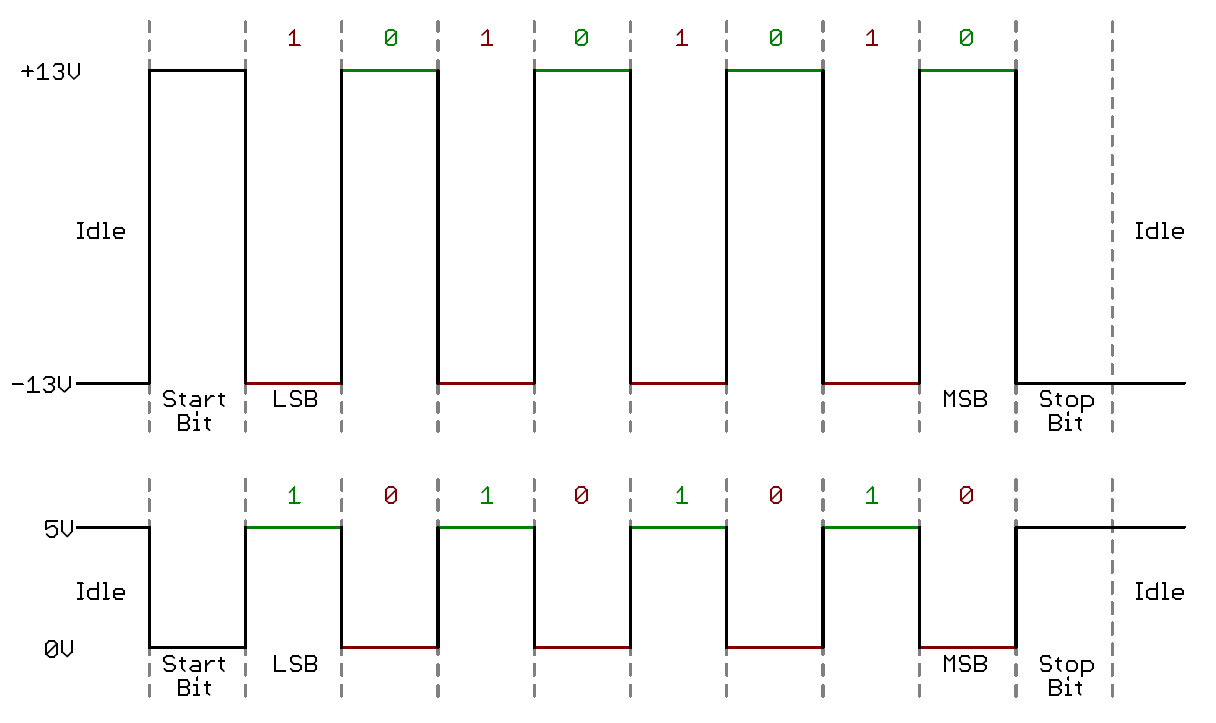
\includegraphics[width=0.9\textwidth]{ttl_rs232.png}}
	\caption{Timing Diagram of RS-232 (top) and TTL Communication Protocols \cite{ttl}}
	\label{ttl_rs232_pic}
\end{figure}

Since these two serial communication formats have incompatible logic levels, an RS-232 to TTL converter is needed so that the rangefinder can communicate with the ZedBoard. The converter's TTL side will be connected to the ZedBoard's Pmod connector, and the RS-232 side will be connected to the rangefinder. However, for ease of connection and testing, the 9-pin DSUB RS-232 connector will be connected to an RS-232 breakout so that the pins can be easily accessed. Figure \ref{rs232_ttl_breakout} shows the RS-232 to TTL converter attached to the RS-232 breakout board.

\begin{figure}[H]
	\centerline{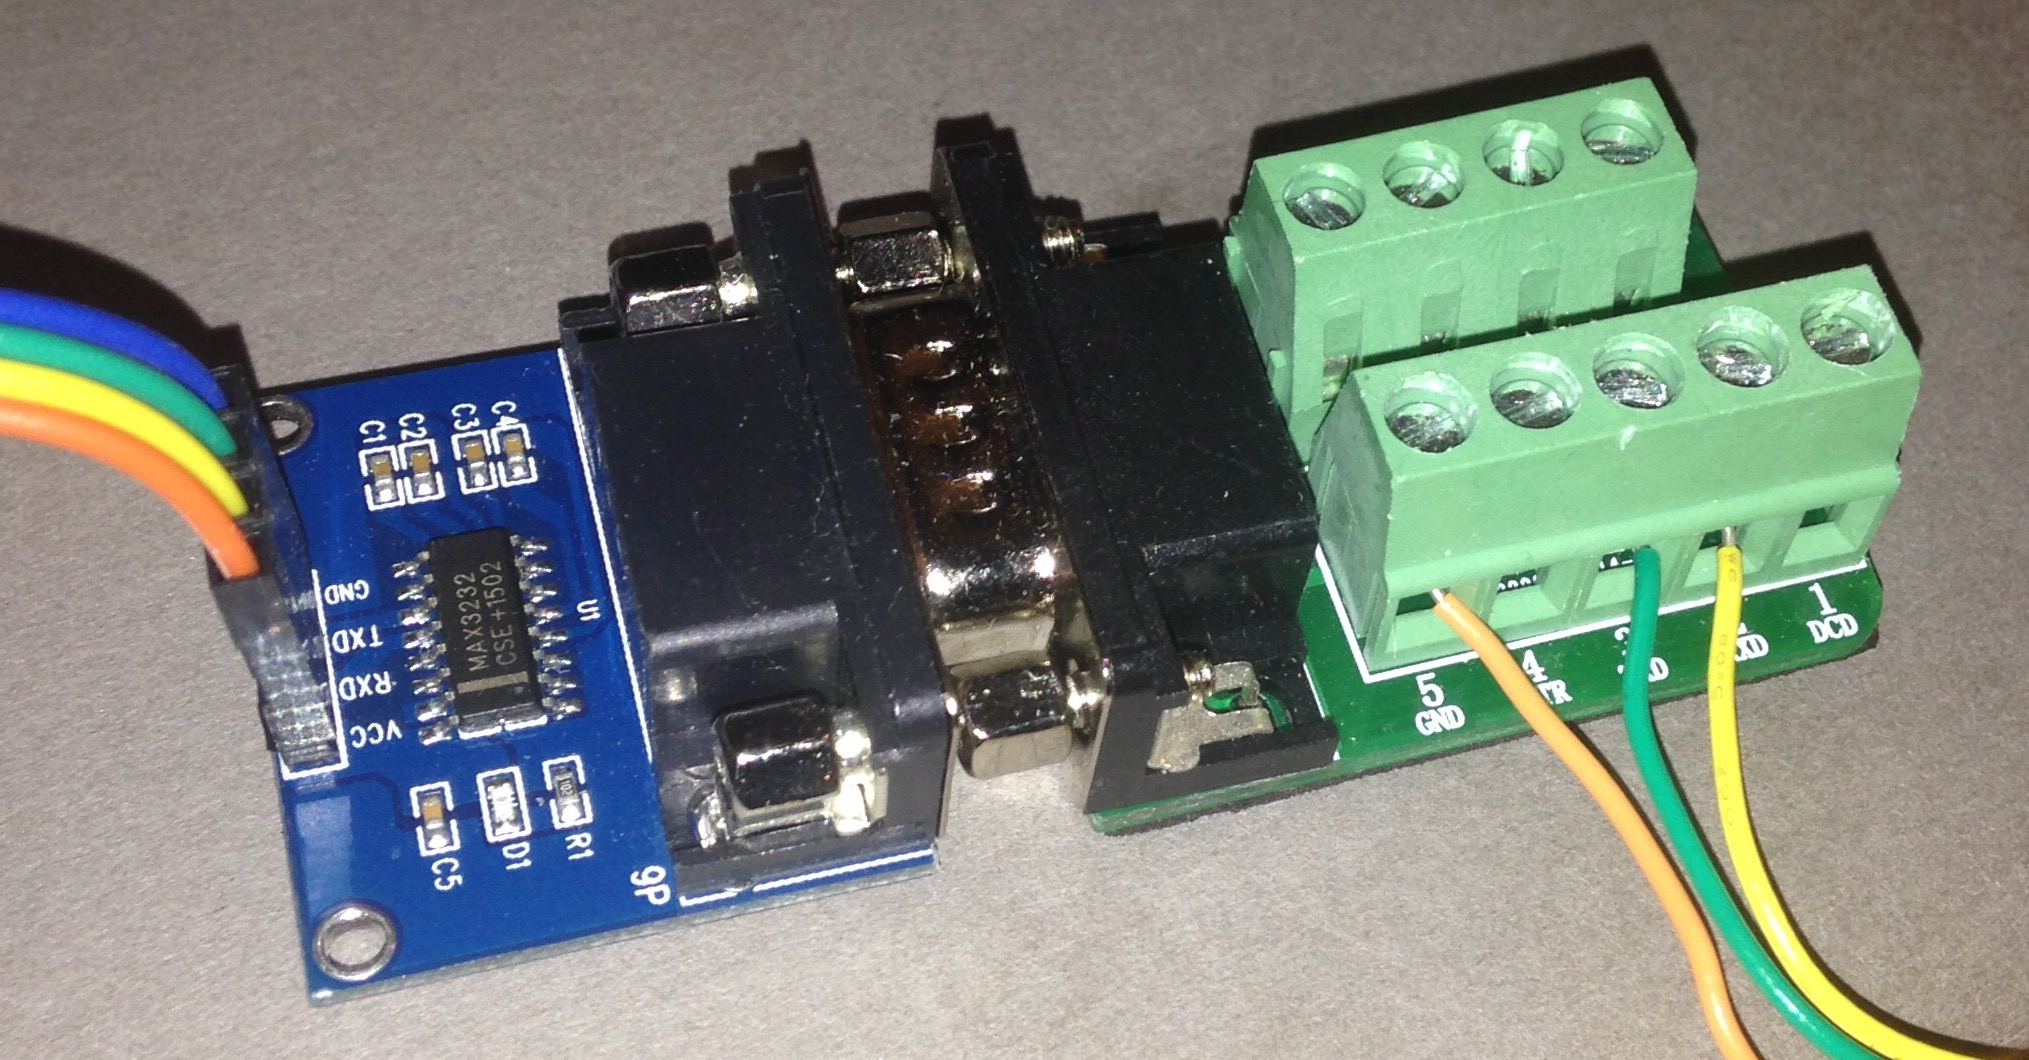
\includegraphics[width=0.5\textwidth]{rs232_ttl_breakout.png}}
	\caption{RS-232 to TTL Converter with RS-232 Breakout Board}
	\label{rs232_ttl_breakout}
\end{figure}

Although the ZedBoard's Pmod connectors are sufficient for UART communication with the URG-04LX, the power specifications are not compatible; the Pmod connectors output 3.3V but the rangefinder requires 5V \cite{zedboard_datasheet, urg04lx_specifications}. Thus, the rangefinder was powered externally by a lab bench power supply.

\subsubsection{Rangefinder Commands}
The rangefinder defaults to a communication speed of 19.2 kbps, or 19200 baud. Using that baud rate over UART, the rangefinder recognizes four different commands: the version command, the laser illumination command, the communication speed setting command, and the distance data acquisition command. The version command is used as a test; as soon as it is received, the rangefinder transmits the device specific information. The laser illumination command is used to turn the laser on and off. The communication speed setting command is used to change the baud rate. The distance data acquisition command is the main command is used to request the distance data from the rangefinder \cite{urg04lx_datasheet}.
\par
The distance data acquisition command is the primary command that will be used for the purpose of this project. This command consists of five different parts that control the data output: 'G', the data starting point, the data end point, the cluster count, and either a line feed or a carriage return. The start point is the step of the area from where the data reading starts, and the end point is the step of the area where the data reading stops. The data reading starts at the start point and traverses counterclockwise until the end point. Changing these steps changes the field of vision of the device. Figure \ref{rangefinder_fov} below shows a top-down view of the device field of vision with the steps labeled.

\begin{figure}[H]
	\centerline{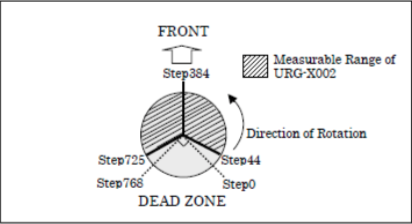
\includegraphics[width=0.7\textwidth]{rangefinder_fov.png}}
	\caption{Top-Down View of Rangefinder Field of Vision \cite{urg04lx_datasheet}}
	\label{rangefinder_fov}
\end{figure}

For this project, we set the beginning point to '000' and the end point to '768' to obtain the device's maximum coverage of 240 degrees. Note that the device's angular rotation per step can be calculated by using Equation \ref{degrees_per_step} below.

\begin{equation}
	360^\circ / 1024 \textrm{ steps}  = 0.3515625^\circ \textrm{ per step}
	\label{degrees_per_step}
\end{equation}

Each step around the rangefinder's field of view corresponds to a change of $0.3515625^\circ$.
\par
The cluster count is the number of neighboring points that are grouped together as a cluster. The cluster count was set to '01' in order to have a cluster count of one data point.
\par
Putting all of these settings together, we get the data acquisition command 'G00076801\textbackslash{}n' which was transmitted from the ZedBoard to the rangefinder to request one cycle of data.

\subsubsection{Rangefinder Testing}
We were able to test the rangefinder by connecting it to a laptop via its USB port. We used PuTTy, a serial console application, to communicate with the rangefinder. Figure \ref{rangefinder_putty} shows the data transfer via PuTTy between a laptop and the rangefinder. Note that PuTTy only shows data received, and that the rangefinder always echoes back the command that it receives.

\begin{figure}[H]
	\centerline{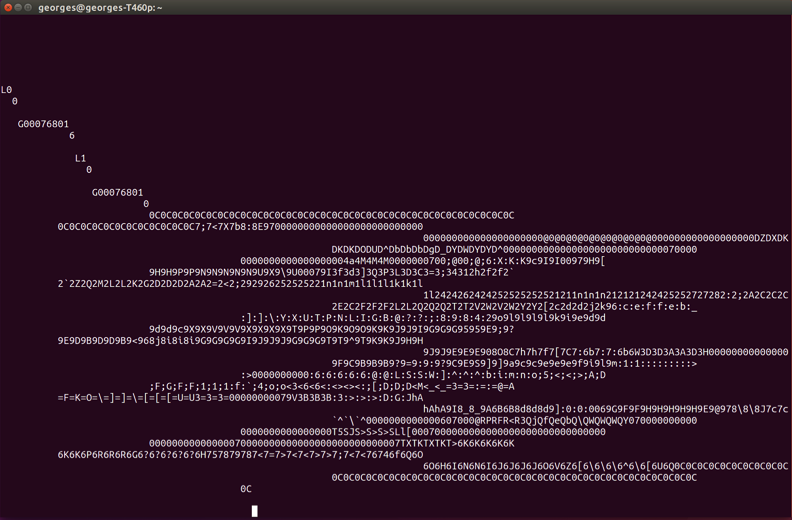
\includegraphics[width=1\textwidth]{rangefinder_putty.png}}
	\caption{Rangefinder Communication Test via PuTTy}
	\label{rangefinder_putty}
\end{figure}

The figure above shows four communication sequences. The first is the laser illumination command 'L0\textbackslash{}n'. Since the laser defaults on, this command turned the laser off. The rangefinder responded to this command first with the echo 'L0\textbackslash{}n', and then with '0', indicating success. The second command is our data acquisition command 'G00076801\textbackslash{}n'. The rangefinder responded with '6', indicating an error code, which was caused by the laser being off. The third command is the laser illumination command again, which turns on the laser. The rangefinder's response was '0' again, indicating success. The last command shown is the data acquisition command again. The rangefinder's response begins with '0', indicating success, followed by the distance data block. The data block consists of 768 points, specified by the data acquisition command. Each data point consists of two characters \cite{urg04lx_datasheet}. By communicating with the rangefinder via PuTTy, we were able to observe the rangefinder's behavior and confirm the data acquisition command functions properly.
\par
In addition to communication via PuTTy, the URG-04LX has a data viewing tool which is a useful application by Hokuyo Automatic that can be used to view, record, and replay the device's data. Again, to use this tool the device must be plugged into a computer via its USB port. Figure \ref{URGBenriStandard_pic} below shows a screen capture of the application recording data captured by the rangefinder.

\begin{figure}[H]
	\centerline{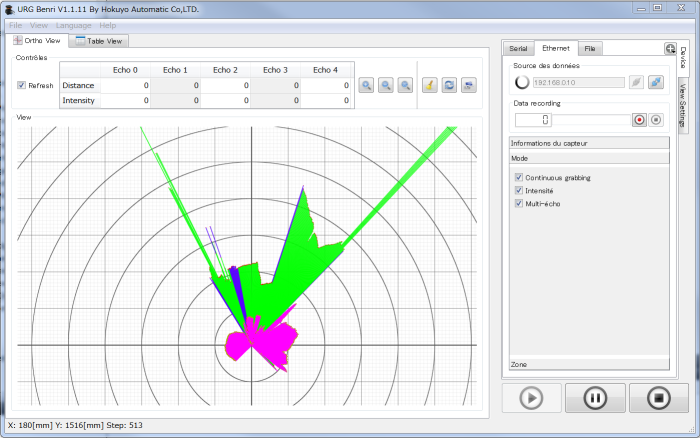
\includegraphics[width=1\textwidth]{UrgBenri_screenshot.png}}
	\caption{Screen Capture of the URG-04LX Data Viewing Tool \cite{URGBenriStandard_ref}}
	\label{URGBenriStandard_pic}
\end{figure}

Note that the start point of 0, end point of 768, and dead zone align to that shown in Figure \ref{rangefinder_fov}. For this project the data viewing tool was used to verify our project's data processing functionality.